\section{Game speed}
Movement is a very important part of any game, but how is movement calculated accurately across different computers?
Different computers have different internals and thus run games with differing performance.
One computer might be able to run the games at 60FPS, but another can only run the game at 30FPS.
How can you make sure that both users have the exact same experience despite the difference in render speed.
A difference in render speed is shown in \autoref{fig:TimeBetweenFramesDisplayed} below.
\begin{figure}[h!]
    \centering
    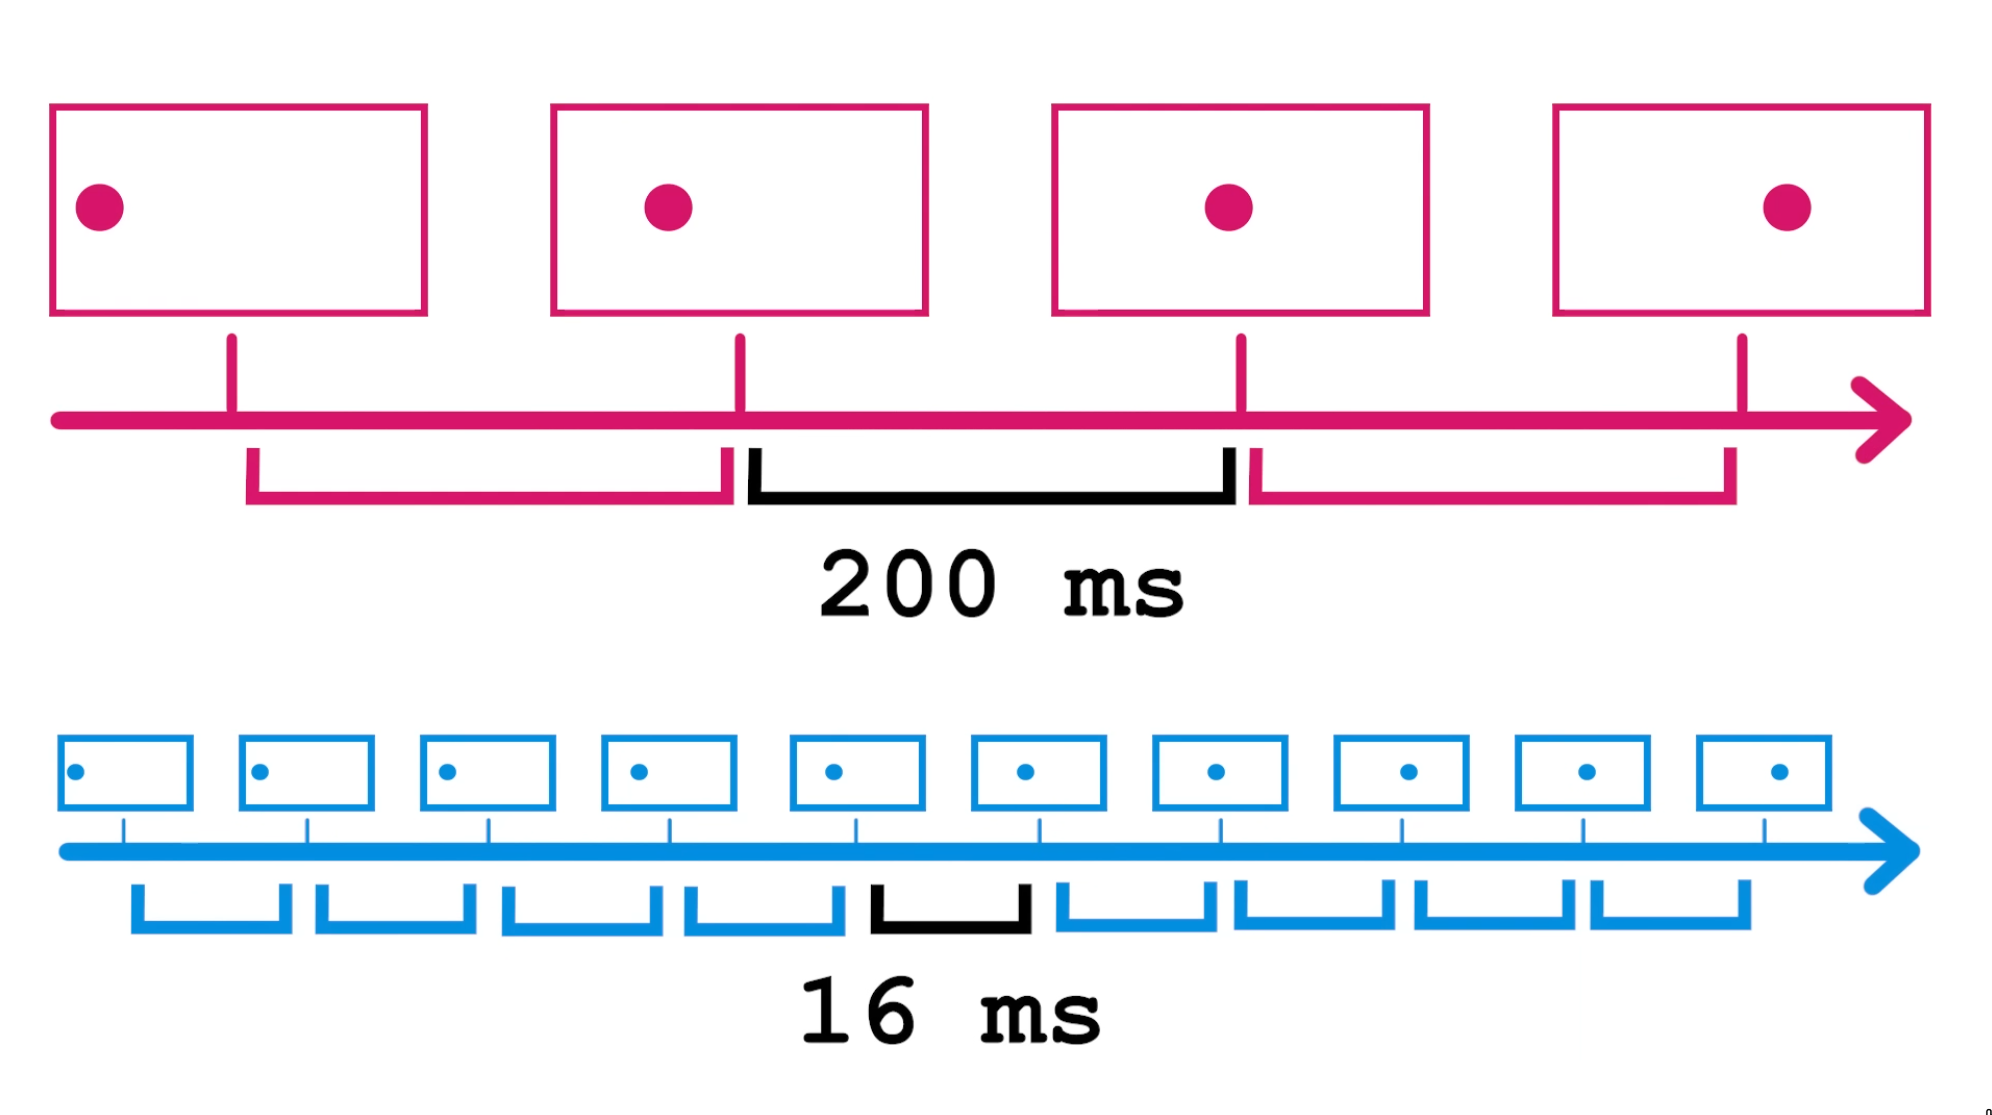
\includegraphics[width=0.8\textwidth]{time_between_frames.png}
    \caption{Time between frames displayed}
    \label{fig:TimeBetweenFramesDisplayed}
\end{figure}

\subsection{Potential problems}
A standard game loop runs one time each frame, before the frame is rendered.
The game loop is responsible for handling all the movement in the game, like moving the player.
If the game runs at 60FPS the game loop will be run 60 times each second.
\newline\newline
The following formula could be used to move the player each game loop iteration:
\newline
playerPosition.x = playerPosition.x + 10
\newline\newline
If this formula would be used to move the player, when running at 60PFS, the player would move 600 units of length each second.
But if the game was running at 30FPS, the player would only move 300 units each second.
So the player with 60FPS is considerably faster than the one with 30FPS.
This is of course, not ideal, as a game developer you want everyone to move at the same speed despite the computer it is run on.
The difference in elapsed distance is also shown in \autoref{fig:DifferenceInElapsedDistance} below.
\begin{figure}[h!]
    \centering
    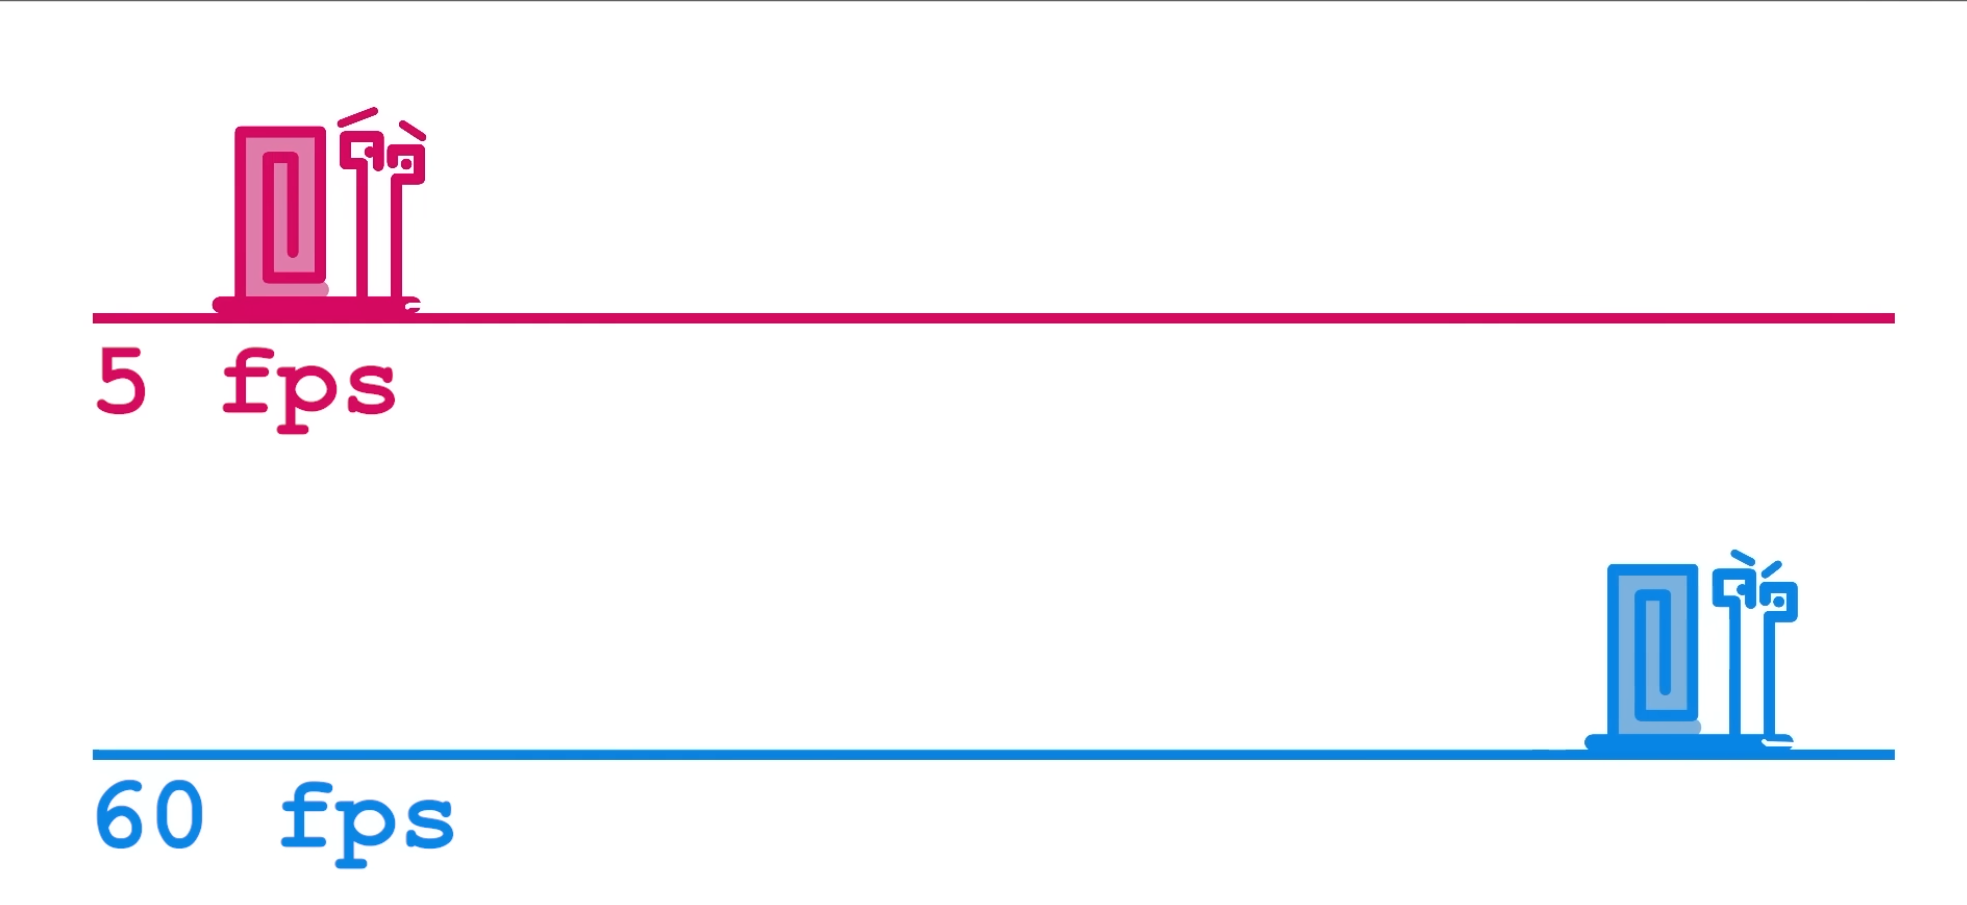
\includegraphics[width=0.8\textwidth]{difference_in_distance.png}
    \caption{Difference in elapsed distance}
    \label{fig:DifferenceInElapsedDistance}
\end{figure}

\subsection{Possible solutions}
There are two common solutions that help alleviate this problem, adjusting the movement speed relative to the FPS or making sure to handle movement in a fixed update loop that is guaranteed to run at a certain amount of cycles each second.

\subsubsection{Fixed update}
A solution to the differing movement speeds between computers, is to create a lightweight time based interrupt, often referred to as FixedUpdate, to handle all movement.
It is important that the FixedUpdate function is very small, otherwise the FixedUpdate could be too slow to be called at a constant rate each frame, defeating the purpose of the FixedUpdate.
In \autoref{fig:FixedUpdateView} below it is shown how times between different rendered frames can vary, while the FixedUpdate is called at a constant rate, where the small black bar represents the duration of the FixedUpdate function.
\begin{figure}[h!]
    \centering
    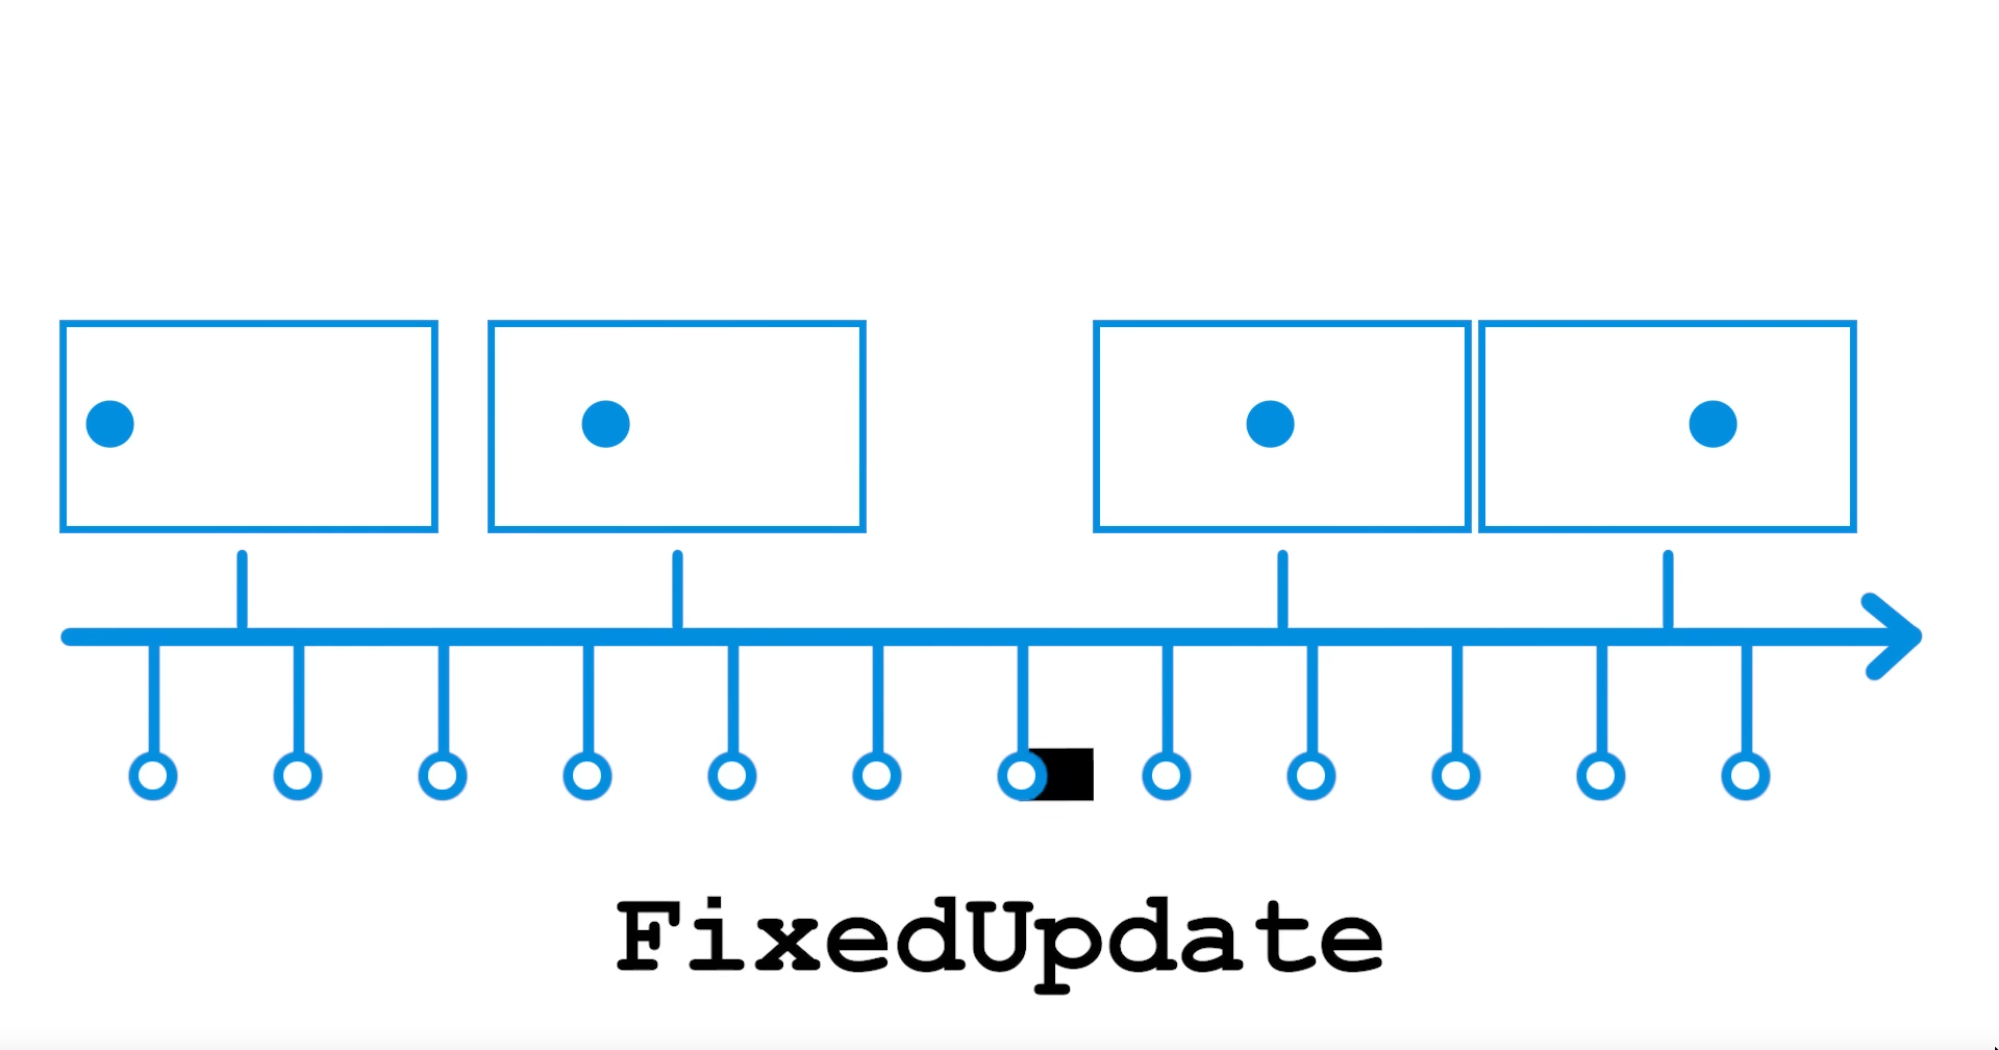
\includegraphics[width=0.6\textwidth]{fixed_update_explanation.png}
    \caption{Fixed update view}
    \label{fig:FixedUpdateView}
\end{figure}
\newline
If you were to use the same formula to calculate the player movement as before, it would now show constant movement between computers.

\subsubsection{Delta time}
Another solution to the differing speeds between computers, is to make the added distance when moving the player relative to the last time distance was added to the player.
Keeping track of every time movement is added to an object is not very efficient so this is solved in a slightly different manner.
So this means the formula would look like this:
\newline
playerPosition.x = playerPosition.x + (10 * deltaTime)
\newline
This uses the deltaTime variable to make the movement relative to the last time the movement was calculated.
\newline\newline
The deltaTime variable is calculated by the game engine and is globally accessible.
The game engine measures the time between the previous frame and the frame before, then assigns that value to the deltaTime variable.
This process is shown in \autoref{fig:DeltaTimeValueWhenUsingVariable}  below where the black square is the place deltaTime is used and the 0.14 is the time it took for the previous frame to render.
\begin{figure}[h!]
    \centering
    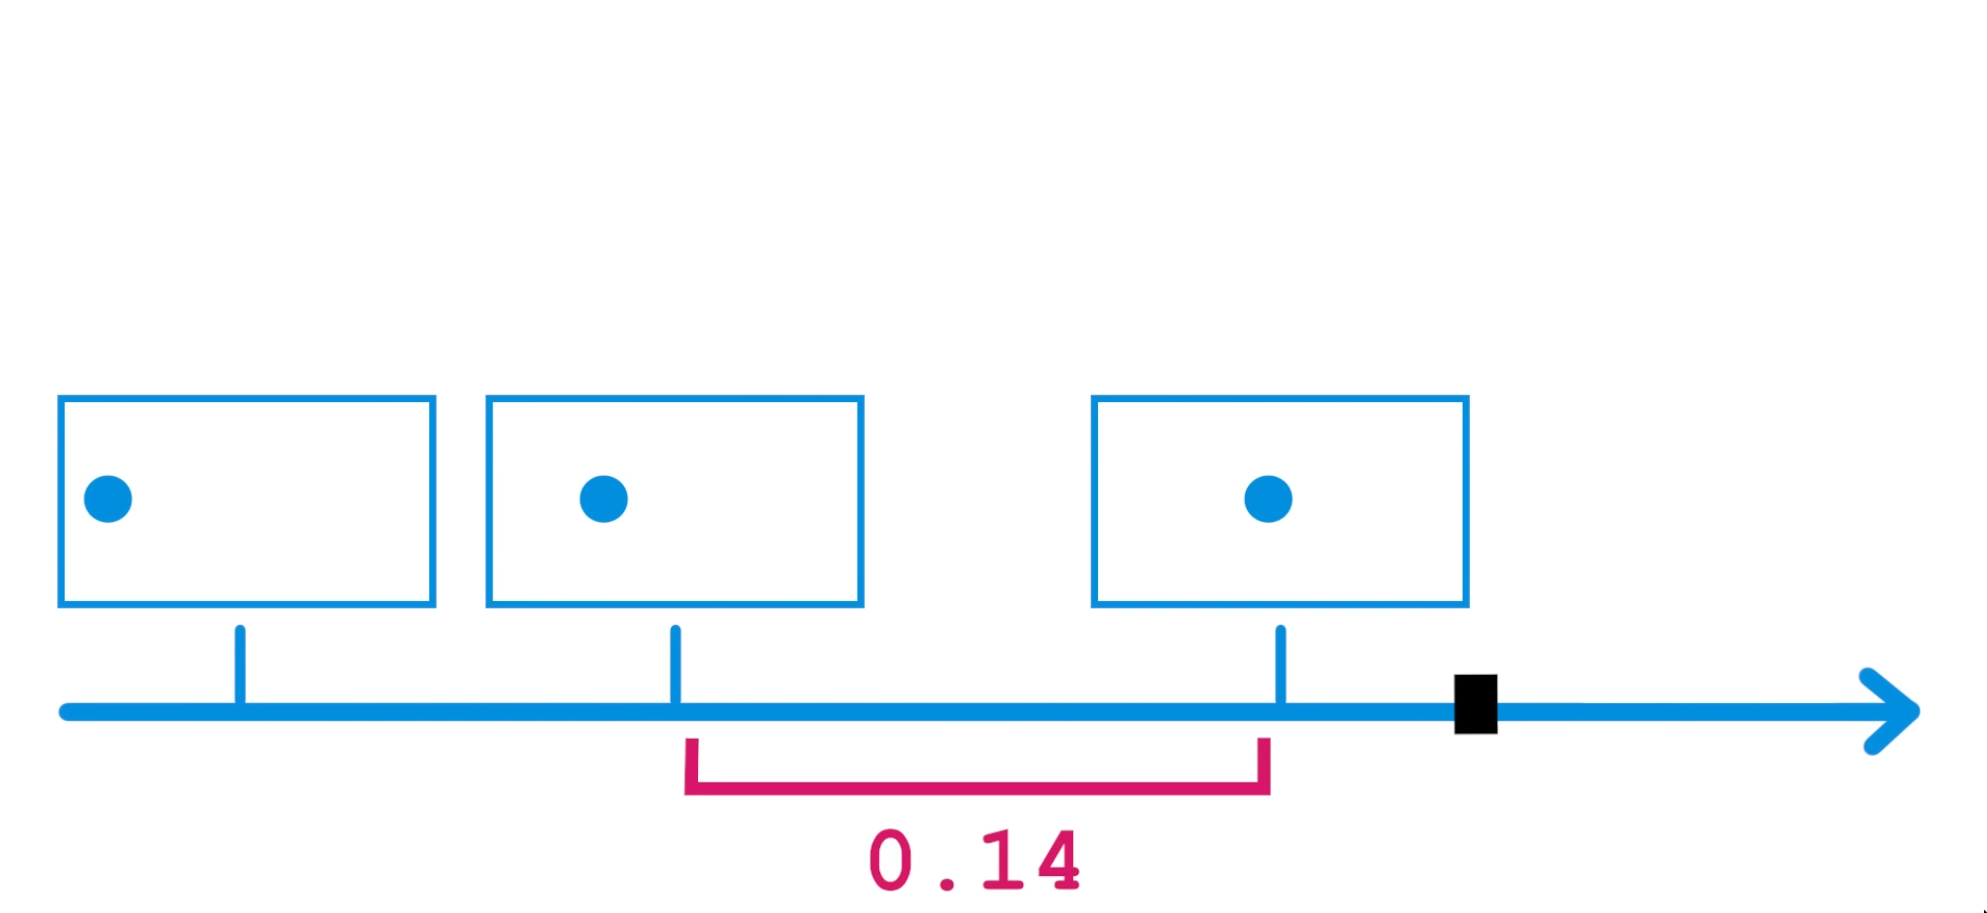
\includegraphics[width=0.6\textwidth]{used_deltatime_when_using_variable.png}
    \caption{deltaTime value when using variable}
    \label{fig:DeltaTimeValueWhenUsingVariable}
\end{figure}
\newline
Because deltaTime is used while rendering a frame, it is not possible to know how long it takes to render the rest of the frame.
This is why the value for the previous frame is used, although this means the deltaTime value lags behind by one frame, the delay is not noticable in most situations.
